\documentclass[12pt]{article}

\usepackage{sbc-template}
\usepackage[T1]{fontenc}
\usepackage[utf8]{inputenc}
\usepackage[brazil]{babel}
\usepackage{graphicx,url}
\usepackage{booktabs}
\usepackage{array}

\sloppy

\title{VacinaBR-PNI: um Dataset Curado e Enriquecido para Análises Epidemiológicas de Doses Aplicadas no Programa Nacional de Imunizações}

\author{Fábio Ribeiro\inst{1}, Andreza Leite\inst{1}}

\address{
  UFRPE\\
  Recife -- PE -- Brasil\\
  \email{fabio.bribeiro@ufrpe.br, andreza.leite@ufrpe.br}
}

\begin{document}

\maketitle

\begin{abstract}
This paper presents VacinaBR-PNI, a curated and enriched dataset derived from open data on vaccine doses administered by the Brazilian National Immunization Program. The dataset was built from monthly CSV files published by the Brazilian Ministry of Health and processed through a reproducible ETL/ELT pipeline. The pipeline standardizes fields, removes sensitive identifiers, derives temporal, geographic and data-quality attributes, stores curated records in Parquet format, and materializes analytical summaries through DuckDB. The resulting dataset supports epidemiological, territorial and data-quality analyses while preserving traceability through metadata, a data dictionary, validation reports, example notebooks and a reproducible publication package.
\end{abstract}

\begin{resumo}
Este artigo apresenta o VacinaBR-PNI, um conjunto de dados curado e enriquecido a partir dos dados abertos de doses aplicadas pelo Programa Nacional de Imunizações. O conjunto de dados foi construído a partir dos arquivos CSV mensais disponibilizados pelo Ministério da Saúde e processado por uma pipeline ETL/ELT reprodutível. A pipeline padroniza campos, remove identificadores sensíveis, deriva atributos temporais, geográficos e de qualidade, armazena os registros curados em formato Parquet e materializa agregados analíticos por meio do DuckDB. O conjunto de dados resultante apoia análises epidemiológicas, territoriais e de qualidade, preservando rastreabilidade por meio de metadados, dicionário de dados, relatórios de validação, notebooks de exemplo e pacote de disponibilização reprodutível.
\end{resumo}

\section{Introdução}

O Programa Nacional de Imunizações (PNI) é uma das principais políticas públicas brasileiras para prevenção e controle de doenças imunopreveníveis. A disponibilidade de dados abertos sobre doses aplicadas permite investigar padrões temporais, territoriais e operacionais da vacinação no Brasil. Esses dados podem apoiar estudos epidemiológicos, análises de cobertura operacional, avaliação de qualidade de registros, construção de painéis públicos e atividades de ensino em ciência de dados aplicada à saúde.

Apesar de sua relevância, os dados brutos publicados pelo Ministério da Saúde não estão imediatamente prontos para uso analítico. Os arquivos mensais possuem grande volume, podem exigir leitura eficiente em partes, contêm campos com potencial sensibilidade, apresentam valores ausentes e demandam padronização de nomes, tipos e categorias. Além disso, pesquisadores frequentemente precisam criar atributos derivados, como ano, mês, trimestre, semana epidemiológica, faixa etária e região geográfica, antes de iniciar análises substantivas.

Este trabalho apresenta o VacinaBR-PNI, um conjunto de dados curado e enriquecido construído a partir dos dados de doses aplicadas do PNI referentes ao ano de 2025. A execução completa contempla os 12 meses do ano, organizados em partições mensais. A principal contribuição é transformar a fonte original em uma camada reutilizável, documentada e consultável, composta por registros curados em Parquet, agregados CSV, uma base DuckDB, dicionário de dados, relatórios de qualidade, notebooks de exemplo e metadados de proveniência. Assim, o projeto aproxima a publicação de dados abertos dos princípios de reuso, interoperabilidade e reprodutibilidade recomendados para artefatos científicos de dados \cite{wilkinson2016fair,peng2011reproducible}.

As contribuições específicas deste trabalho são: (i) uma pipeline reprodutível de coleta, tratamento e validação; (ii) uma camada processada sem campos sensíveis diretos; (iii) indicadores de qualidade por mês, unidade federativa e vacina; (iv) enriquecimento geográfico por município; e (v) artefatos de disponibilização voltados ao reuso acadêmico.

\section{Trabalhos Relacionados}

Iniciativas de dados abertos em saúde têm papel relevante na transparência pública, no monitoramento epidemiológico e no desenvolvimento de pesquisas reprodutíveis. No contexto brasileiro, o Portal de Dados Abertos do SUS disponibiliza bases relacionadas a imunização, atendimento, vigilância e outros processos do sistema de saúde \cite{datasus_pni_2025}. Embora essas fontes sejam fundamentais, seu uso direto frequentemente exige etapas de engenharia de dados, padronização, validação e documentação.

A literatura sobre dados científicos enfatiza que conjuntos de dados reutilizáveis devem ser acompanhados de metadados, documentação, identificadores persistentes e critérios claros de proveniência. Os princípios FAIR propõem que dados sejam encontráveis, acessíveis, interoperáveis e reutilizáveis \cite{wilkinson2016fair}. De modo complementar, discussões sobre pesquisa computacional reprodutível destacam a importância de disponibilizar código, dados e procedimentos capazes de reconstruir os resultados \cite{peng2011reproducible}.

Artigos de dados também cumprem papel importante ao documentar o contexto de produção, a estrutura, a qualidade e o potencial de reuso de um conjunto de dados \cite{chavan2011data}. Em comparação com a publicação bruta de arquivos transacionais, a curadoria agrega valor ao documentar o esquema, remover informações sensíveis, criar atributos derivados, explicitar critérios de qualidade e fornecer formatos eficientes de armazenamento. O VacinaBR-PNI se insere nesse contexto como um conjunto de dados derivado dos dados abertos do PNI, com foco em reprodutibilidade, consulta analítica e reuso em pesquisas.

\section{Metodologia de Coleta e Processamento}

\subsection{Fontes de Dados}

A fonte primária é composta pelos arquivos CSV mensais de doses aplicadas pelo Programa Nacional de Imunizações, publicados no Portal de Dados Abertos do SUS \cite{datasus_pni_2025}. Cada arquivo mensal é distribuído em formato compactado e contém registros individuais de aplicação de vacinas ou imunobiológicos. No projeto, esses arquivos são descritos por um manifesto de coleta, que registra o mês, a URL de origem, o nome esperado do arquivo e o status de processamento. Esse manifesto também permite reexecutar a coleta de modo controlado, seja para apenas um mês de teste, seja para a execução completa dos 12 meses.

Como fonte auxiliar, utiliza-se a API de Localidades do IBGE para enriquecimento geográfico municipal \cite{ibge_localidades}. Essa etapa permite associar códigos municipais a metadados de município, unidade federativa e região, além de coordenadas geográficas auxiliares utilizadas nas visualizações cartográficas. O enriquecimento não altera o conteúdo original dos registros de vacinação; ele adiciona contexto territorial para consultas, mapas e análises espaciais.

\subsection{Pipeline ETL/ELT}

A pipeline foi implementada em Python e projetada para execução em Google Colab com armazenamento persistente no Google Drive. Essa escolha facilita a reprodução do processamento em ambiente acessível, sem necessidade de infraestrutura local robusta. O fluxo principal contempla as seguintes etapas:

\begin{enumerate}
    \item definição de um manifesto com os arquivos mensais oficiais;
    \item download dos arquivos ZIP para a camada bruta;
    \item leitura incremental dos CSVs em lotes (\textit{chunks});
    \item atribuição do esquema posicional quando os arquivos não possuem cabeçalho;
    \item padronização de nomes de colunas e aliases operacionais;
    \item conversão de tipos, normalização textual e tratamento de valores ausentes;
    \item remoção de campos sensíveis, como identificadores de paciente e CEP;
    \item derivação de atributos temporais, territoriais e de qualidade;
    \item verificação de duplicatas por assinatura de linha;
    \item escrita dos registros curados em Parquet, particionados por ano e mês;
    \item criação de uma camada DuckDB para consultas SQL e agregados analíticos;
    \item geração de CSVs sumarizados, dicionário de dados, relatórios de validação e metadados.
\end{enumerate}

\begin{figure}[ht]
\centering
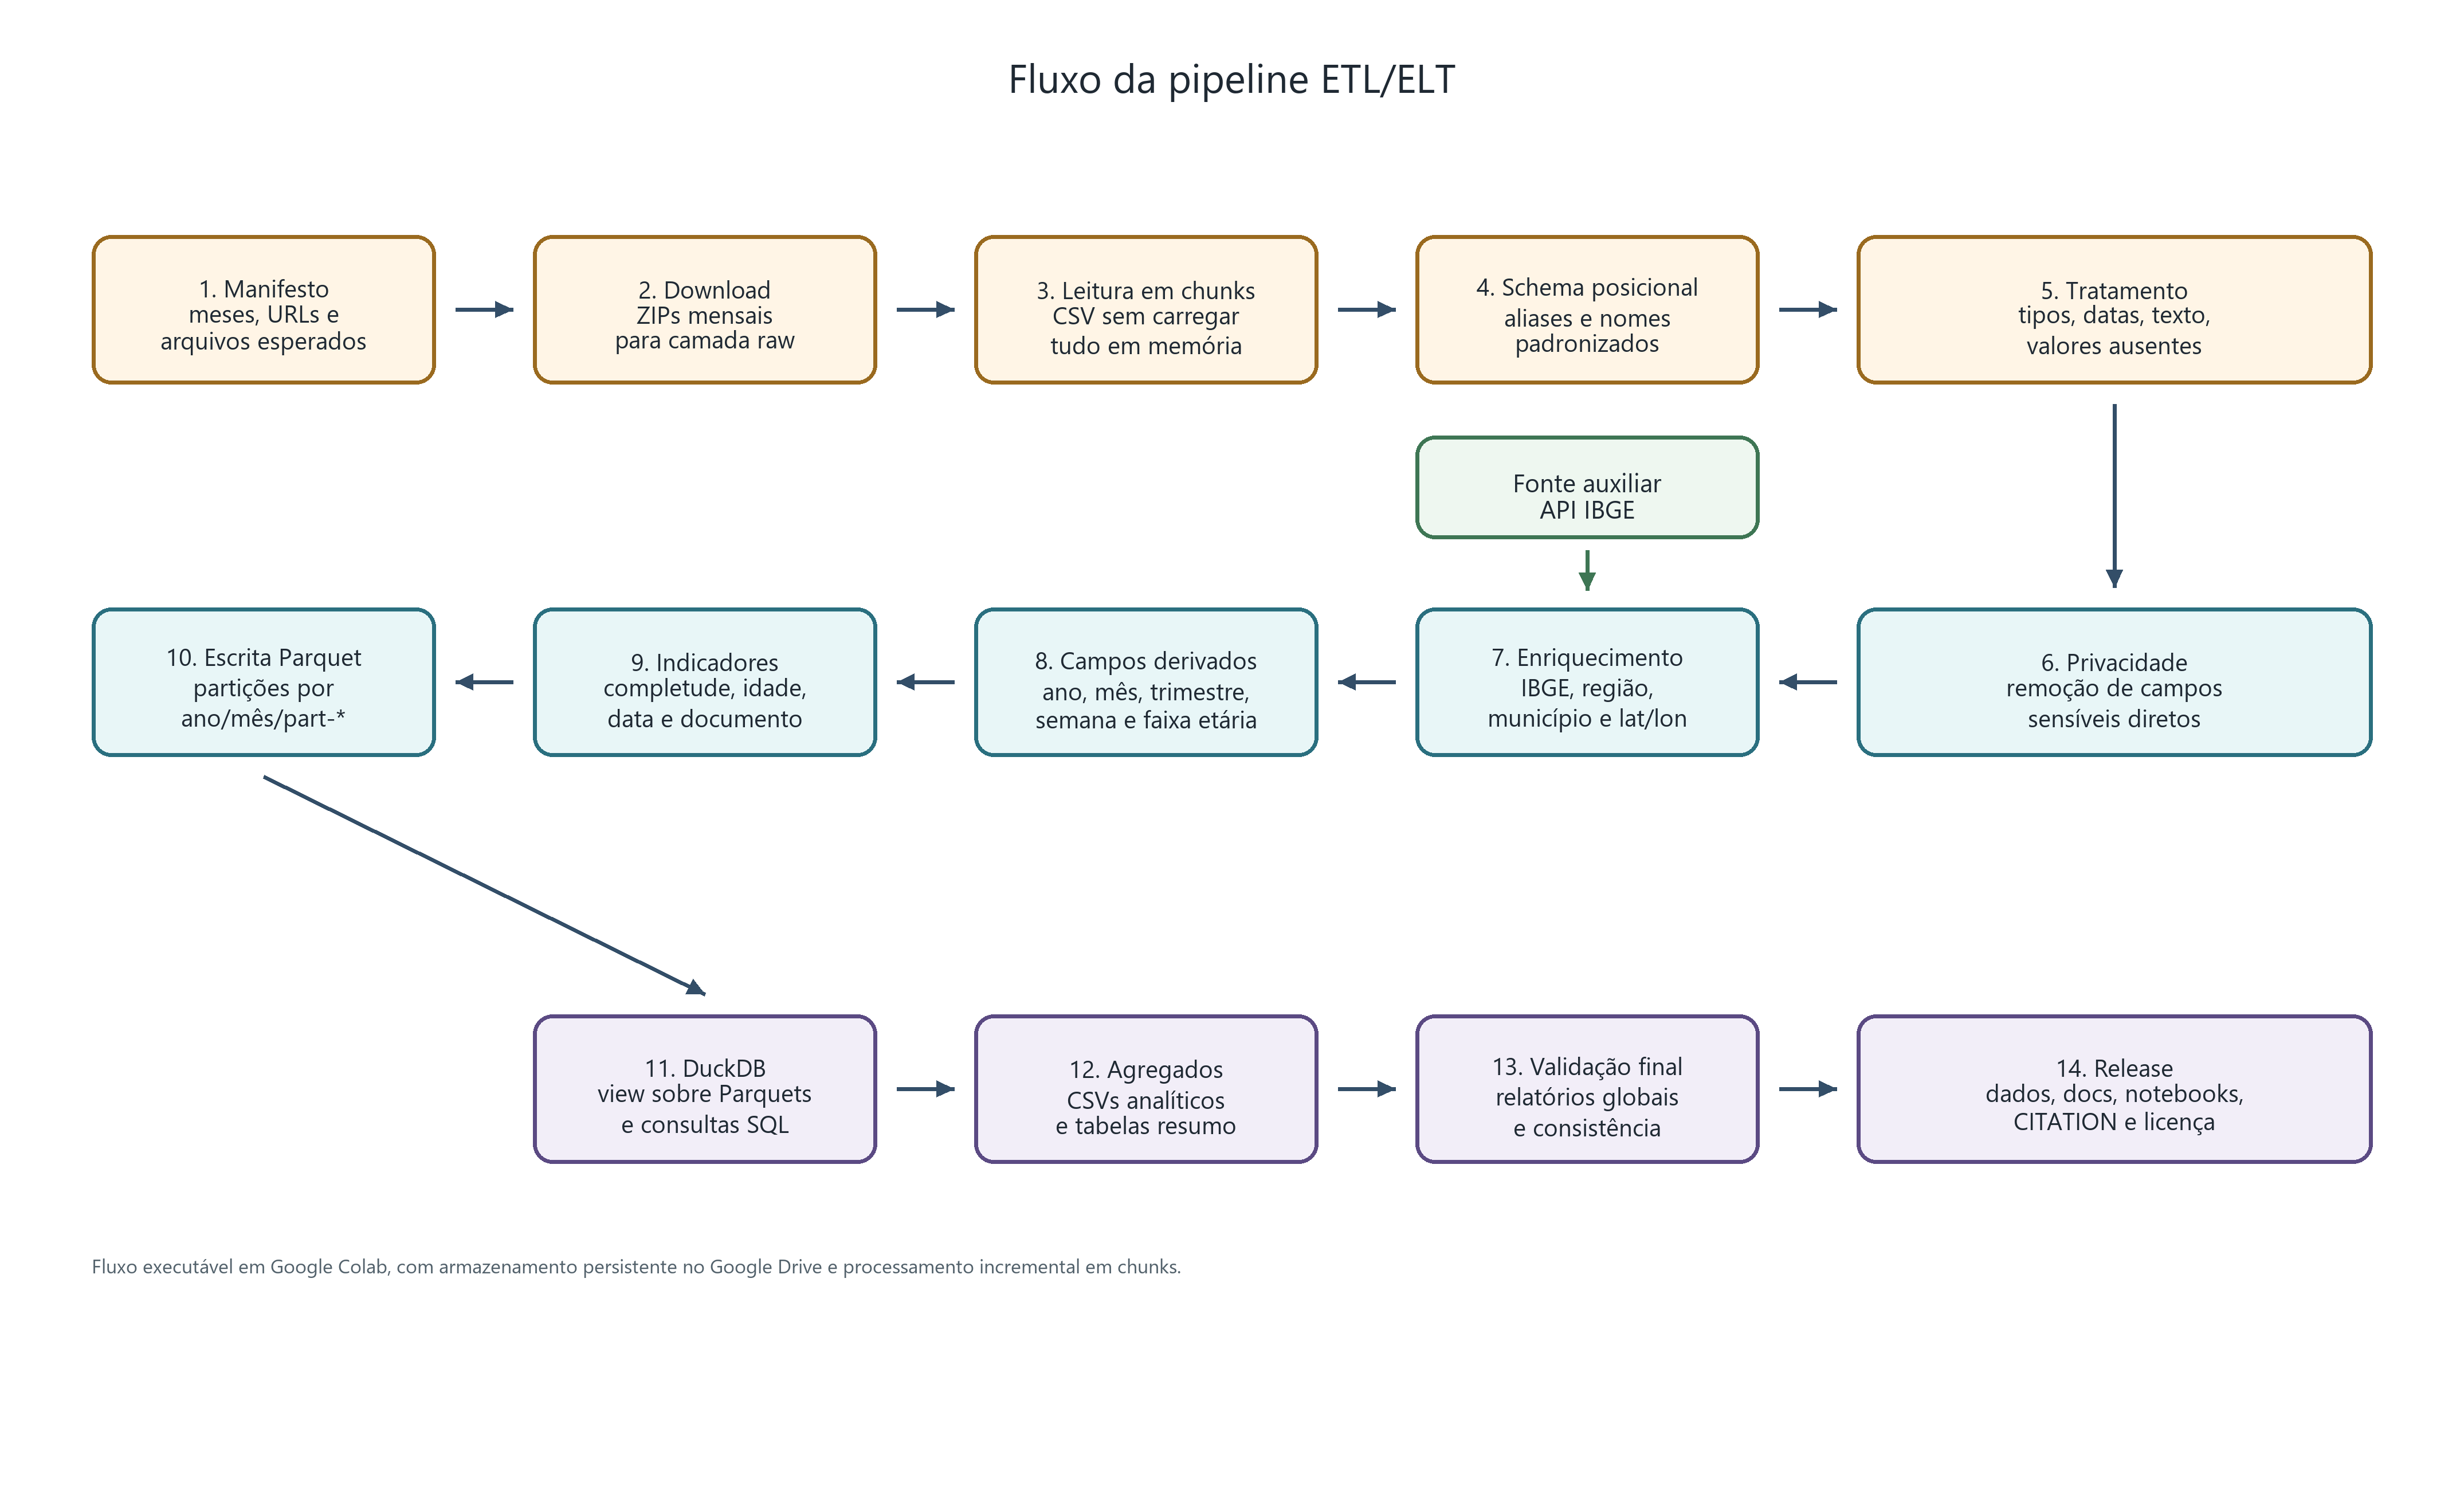
\includegraphics[width=0.95\linewidth]{figures/pipeline_flow.png}
\caption{Fluxo operacional da pipeline ETL/ELT, desde o manifesto de coleta até a geração dos artefatos de disponibilização.}
\label{fig:pipeline-flow}
\end{figure}

A leitura em lotes (\textit{chunks}) foi adotada para reduzir o consumo de memória durante o processamento de arquivos grandes, especialmente no ambiente Google Colab. Cada lote tratado é gravado como um arquivo Parquet independente, com nomes do tipo \texttt{part-*}. Assim, um mesmo mês pode gerar múltiplos arquivos dentro da mesma partição, sem que isso altere o modelo lógico do conjunto de dados. Para o usuário final, esses arquivos podem ser consultados como uma única tabela por ferramentas compatíveis com Parquet, como o DuckDB. O formato Parquet foi escolhido por oferecer armazenamento colunar eficiente, compressão e leitura seletiva de colunas, características adequadas a cargas analíticas \cite{apache_parquet}. O DuckDB foi utilizado como banco analítico embarcado para consulta direta aos Parquets e materialização de tabelas resumo \cite{duckdb}.

\subsection{Tratamento, Padronização e Campos Derivados}

A etapa de tratamento converte campos de data, idade e códigos geográficos para tipos consistentes. Também normaliza valores textuais para reduzir diferenças causadas por acentuação, caixa ou espaços excedentes. Campos ausentes são preservados quando representam ausência real de informação, mas são contabilizados nos relatórios de qualidade.

A pipeline cria atributos derivados que facilitam consultas comuns. Por exemplo, a partir de \texttt{data\_vacina = 2025-01-14}, são gerados \texttt{ano\_vacinacao = 2025}, \texttt{mes\_vacinacao = 1}, \texttt{trimestre\_vacinacao = Q1} e \texttt{semana\_epidemiologica = 3}. A partir de \texttt{numero\_idade\_paciente = 59}, são gerados \texttt{faixa\_etaria = 40-59} e \texttt{idade\_valida = true}. A partir de \texttt{uf\_paciente = SP}, é gerado \texttt{regiao\_paciente = Sudeste}. Esses campos reduzem o esforço de preparação por parte do usuário final.

\subsection{Fluxo de Dados e Artefatos}

O fluxo de dados do projeto está organizado em camadas. A camada bruta preserva os arquivos ZIP originais. A camada processada armazena os registros curados em Parquet, particionados por ano e mês. Dentro de cada partição mensal, os arquivos \texttt{part-*} refletem o processamento incremental em lotes. A camada analítica contém CSVs agregados para exploração rápida, uso em planilhas e ferramentas de BI. A camada DuckDB fornece uma interface SQL sobre os Parquets e materializa tabelas de resumo. Por fim, a camada documental contém dicionário de dados, esquema, relatório de validação, catálogo DuckDB e metadados da fonte.

\begin{figure}[ht]
\centering
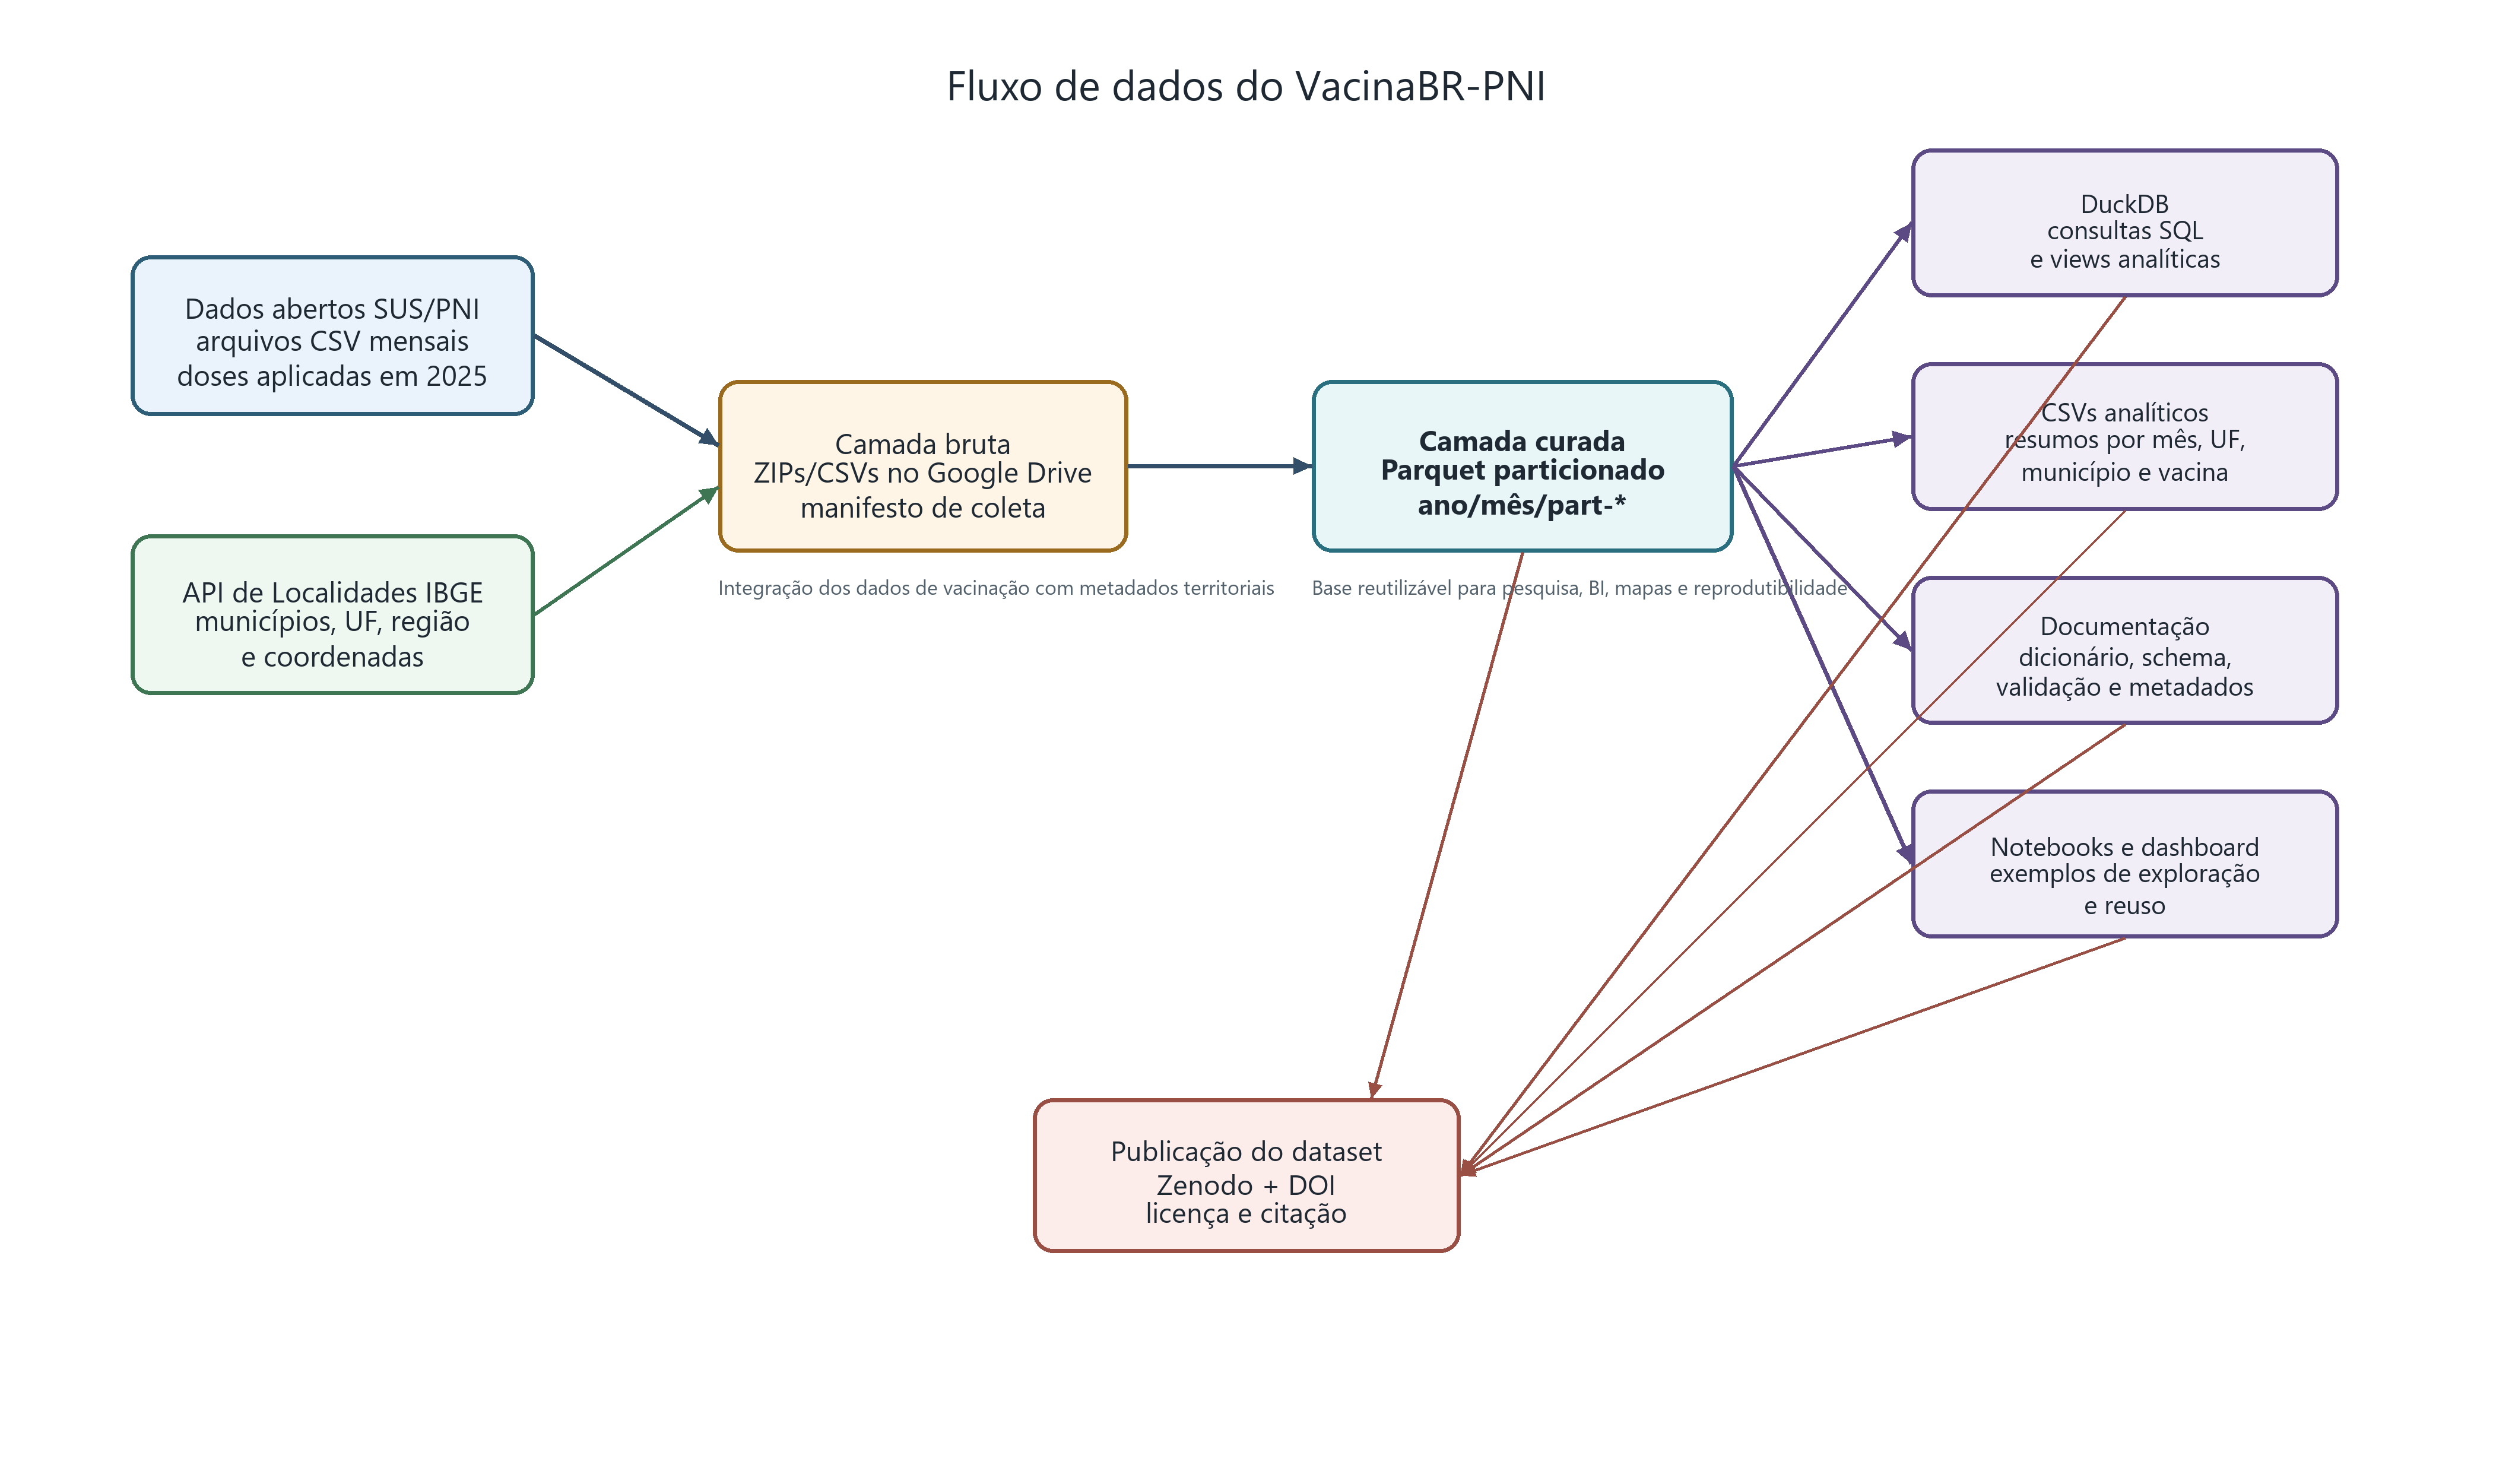
\includegraphics[width=0.95\linewidth]{figures/data_flow.png}
\caption{Fluxo de dados do VacinaBR-PNI, incluindo a fonte primária do PNI, a fonte auxiliar do IBGE, as camadas de armazenamento e os artefatos de reuso e publicação.}
\label{fig:data-flow}
\end{figure}

\begin{table}[ht]
\centering
\caption{Camadas do fluxo de dados do VacinaBR-PNI.}
\label{tab:storage-layers}
\begin{tabular}{p{3cm}p{9cm}}
\toprule
\textbf{Camada} & \textbf{Descrição} \\
\midrule
Raw & Arquivos ZIP mensais originais baixados do Portal de Dados Abertos do SUS. \\
Processed & Arquivos Parquet curados, particionados por ano e mês, com múltiplos arquivos \texttt{part-*} por partição quando necessário. \\
Analytics & CSVs agregados por mês, UF, região, município, vacina, fabricante, sexo, faixa etária e qualidade. \\
DuckDB & Banco analítico embarcado com visões e tabelas materializadas. \\
Docs & Dicionário de dados, esquema, validação, catálogo e metadados de proveniência. \\
\bottomrule
\end{tabular}
\end{table}

\section{Descrição do Dataset}

\subsection{Estrutura}

O conjunto de dados tem como entidade central o registro de dose aplicada. Cada registro representa uma aplicação de vacina ou imunobiológico, associada a atributos do paciente, estabelecimento, vacina, dose, data, município, unidade federativa, sistema de origem e status documental. A partir dessa entidade principal, o processamento produz dimensões e agregados analíticos relacionados a tempo, território, vacina, fabricante e qualidade.

Além da tabela curada em nível de registro, o projeto gera uma dimensão auxiliar de vacinas, representada por \texttt{vaccine\_dictionary.csv}, e uma dimensão geográfica municipal, representada no DuckDB por \texttt{municipality\_geography}. Os agregados analíticos permitem consultas sem necessidade de percorrer todos os registros individuais, o que torna o conjunto de dados mais acessível para usuários de planilhas, BI e notebooks.

\begin{figure}[ht]
\centering
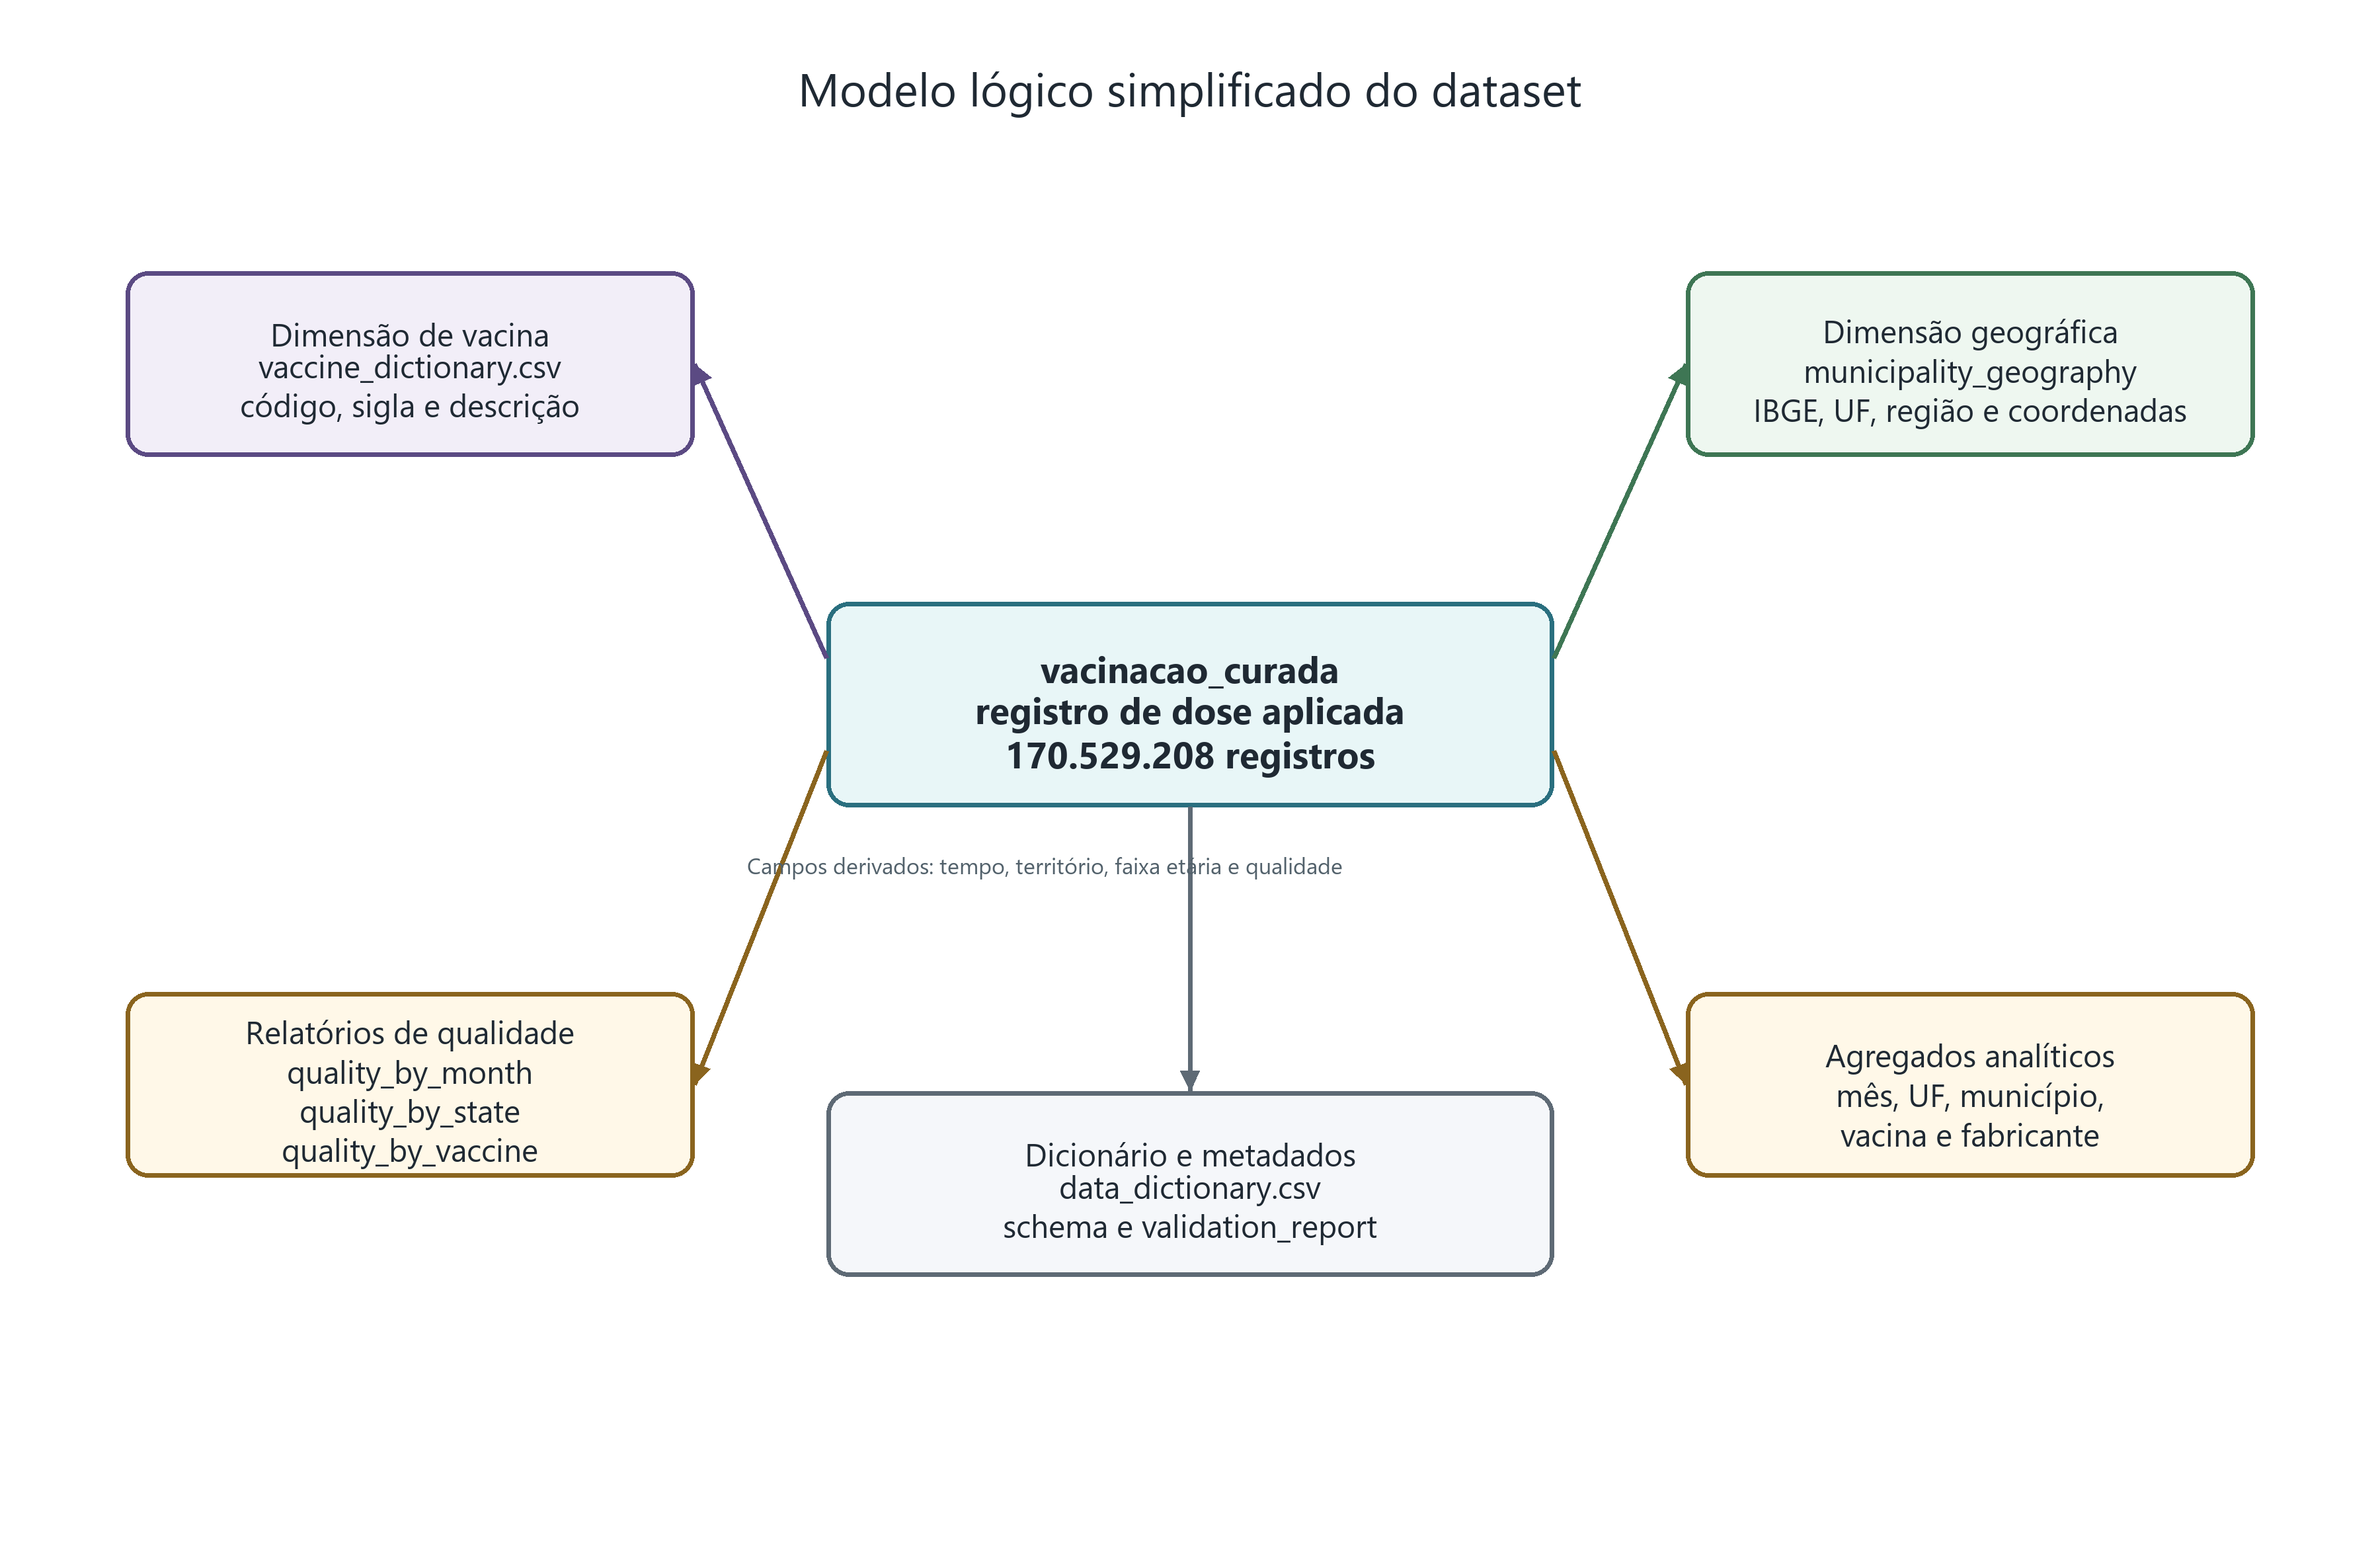
\includegraphics[width=0.90\linewidth]{figures/dataset_model.png}
\caption{Modelo lógico simplificado do conjunto de dados.}
\label{fig:dataset-model}
\end{figure}

\subsection{Esquema de Dados}

O esquema curado preserva campos relevantes da fonte original e acrescenta atributos derivados. Entre os atributos preservados estão \texttt{data\_vacina}, \texttt{sexo\_paciente}, \texttt{numero\_idade\_paciente}, \texttt{uf\_paciente}, \texttt{codigo\_municipio\_paciente}, \texttt{codigo\_vacina}, \texttt{sg\_vacina}, \texttt{descricao\_vacina}, \texttt{descricao\_dose\_vacina} e \texttt{descricao\_vacina\_fabricante}. Entre os atributos derivados estão \texttt{ano\_vacinacao}, \texttt{mes\_vacinacao}, \texttt{trimestre\_vacinacao}, \texttt{semana\_epidemiologica}, \texttt{faixa\_etaria}, \texttt{regiao\_paciente}, \texttt{idade\_valida}, \texttt{registro\_completo} e \texttt{registro\_valido\_documento}.

\begin{table}[ht]
\centering
\caption{Principais atributos do conjunto de dados curado.}
\label{tab:main-attributes}
\begin{tabular}{p{4.8cm}p{1.8cm}p{4.9cm}}
\toprule
\textbf{Atributo} & \textbf{Origem} & \textbf{Uso analítico} \\
\midrule
\texttt{data\_vacina} & Fonte & Análise temporal da aplicação. \\
\texttt{uf\_paciente} & Fonte & Agregação estadual. \\
\texttt{codigo\_municipio\_}\\
\texttt{paciente} & Fonte & Agregação municipal e junção geográfica. \\
\texttt{sg\_vacina} & Fonte & Agrupamento por tipo de vacina. \\
\texttt{descricao\_vacina} & Fonte & Interpretação textual da vacina. \\
\texttt{faixa\_etaria} & Derivado & Análise por grupos etários. \\
\texttt{regiao\_paciente} & Derivado & Análise regional. \\
\texttt{registro\_completo} & Derivado & Indicador de completude. \\
\texttt{registro\_valido\_}\\
\texttt{documento} & Derivado & Indicador de validade documental. \\
\bottomrule
\end{tabular}
\end{table}

\subsection{Dicionário de Dados}

O dicionário de dados é disponibilizado no arquivo \texttt{docs/data\_dictionary.csv}. Ele descreve o nome do campo, tipo, descrição, origem, exemplo de valor e indicação de sensibilidade. Essa documentação apoia a interpretação por usuários externos, reduz ambiguidade sobre campos derivados e torna explícita a diferença entre atributos preservados da fonte e atributos produzidos pela curadoria.

\subsection{Volumetria}

A pipeline registra métricas como quantidade de registros originais, registros processados, duplicatas removidas, número de colunas, valores ausentes, registros completos, registros incompletos, idades inválidas, datas inválidas e documentos válidos. Na execução completa de 2025, foram lidos 170.529.208 registros brutos e o mesmo total foi preservado na camada processada, sem remoção de duplicatas. Esse resultado indica que, para a rodada considerada, não houve perda de registros durante o processamento.

Também foram identificados 1.541.678.848 valores ausentes no conjunto processado. Essa métrica representa a soma de ausências em todas as colunas avaliadas e, portanto, não corresponde ao número de registros incompletos. Em nível de registro, 111.176.188 observações foram classificadas como completas, enquanto 59.353.020 apresentaram ausência em pelo menos um campo essencial avaliado pela pipeline.

\begin{table}[ht]
\centering
\caption{Volumetria da execução analisada.}
\label{tab:volumetry}
\begin{tabular}{p{6.3cm}p{4.5cm}}
\toprule
\textbf{Métrica} & \textbf{Valor} \\
\midrule
Registros brutos & 170.529.208 \\
Registros processados & 170.529.208 \\
Duplicatas removidas & 0 \\
Valores ausentes totais & 1.541.678.848 \\
Registros completos & 111.176.188 \\
Registros incompletos & 59.353.020 \\
Arquivos Parquet gerados & 1.712 \\
Tamanho da camada Parquet & 12.048,45 MB \\
Municípios observados & 5.623 \\
Siglas de vacina observadas & 108 \\
\bottomrule
\end{tabular}
\end{table}

\begin{figure}[ht]
\centering
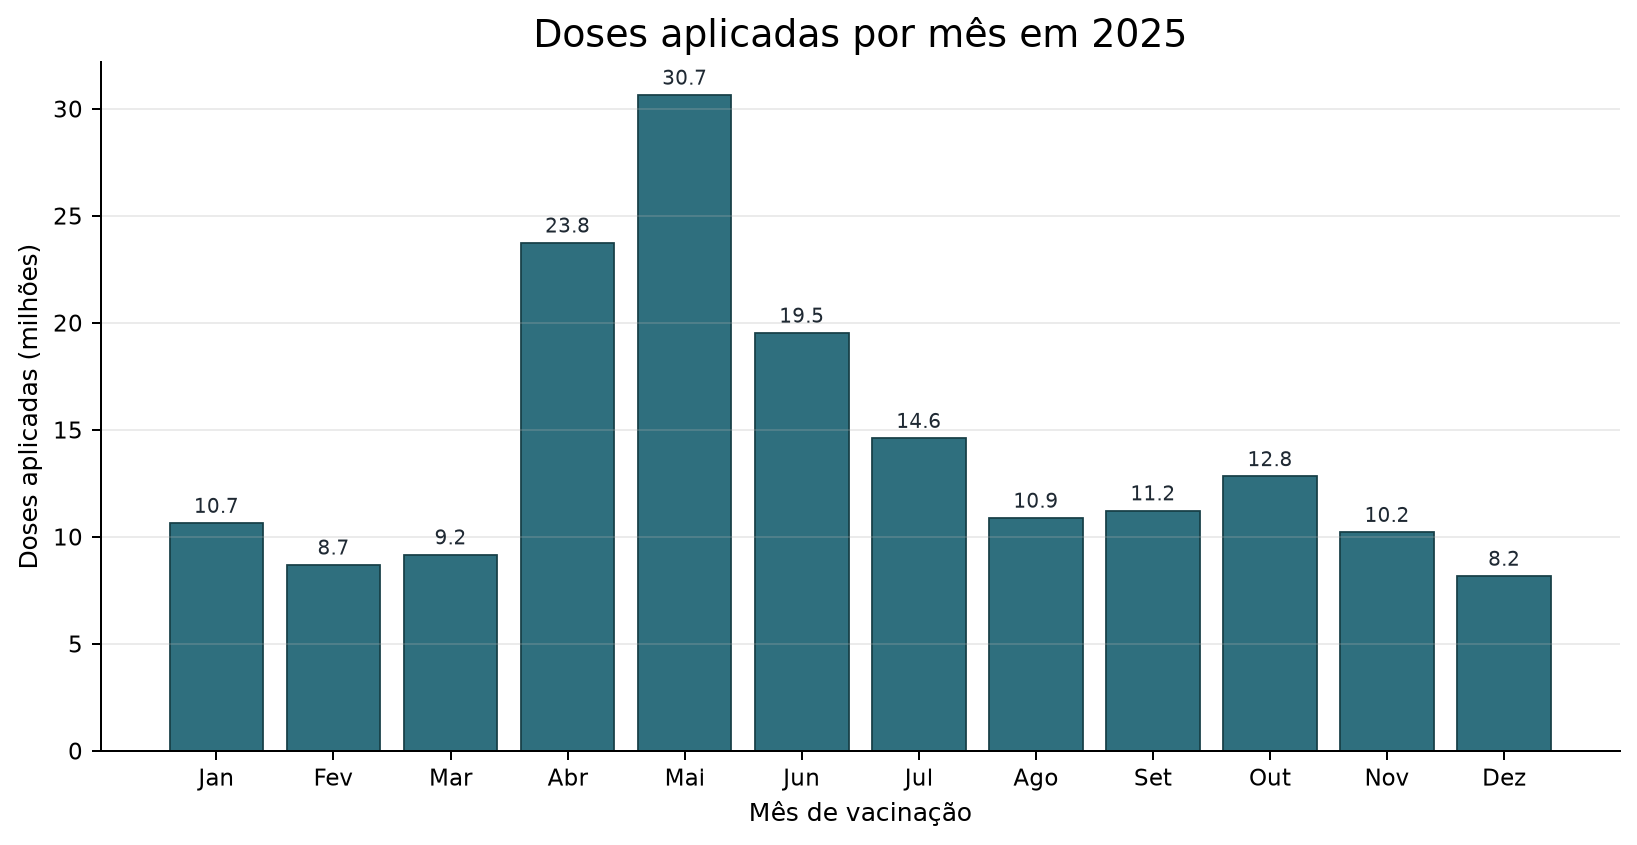
\includegraphics[width=0.90\linewidth]{figures/monthly_volumetry.png}
\caption{Volumetria mensal de doses aplicadas.}
\label{fig:monthly-volumetry}
\end{figure}

\subsection{Formatos de Armazenamento}

O conjunto de dados é disponibilizado em múltiplos formatos para atender diferentes usos. Os arquivos Parquet constituem a camada principal de pesquisa, pois preservam registros curados em formato colunar eficiente. Eles são particionados por ano e mês, o que permite consultar apenas o período necessário, sem carregar a base inteira. Na execução completa, a camada processada gerou 1.712 arquivos Parquet, totalizando 12.048,45 MB. Esse volume é compatível com publicação em repositórios de dados, mas inadequado para versionamento direto em GitHub.

Os CSVs analíticos permitem uso direto em planilhas, painéis e ferramentas de visualização. O arquivo DuckDB oferece uma camada SQL portátil, sem necessidade de servidor, adequada para consultas exploratórias e reprodução de resultados. Por exemplo, um usuário pode consultar todos os Parquets com uma expressão como \texttt{read\_parquet('data/processed/**/*.parquet')} ou filtrar apenas um mês específico pela partição correspondente. A documentação e os notebooks complementam esses formatos ao explicar o significado dos campos e demonstrar formas de consulta.

\section{Validação Técnica e Qualidade}

A qualidade dos dados foi assegurada por validações automatizadas durante e após o processamento. A pipeline verifica o esquema, padroniza nomes de colunas, converte tipos, remove campos sensíveis, calcula indicadores de completude e cria marcadores de qualidade documental. Campos como \texttt{codigo\_paciente} e \texttt{numero\_cep\_paciente} são removidos da camada processada, reduzindo riscos de exposição de informações pessoais e alinhando o conjunto de dados a práticas de minimização de dados \cite{lgpd}.

As verificações implementadas incluem validação de colunas esperadas, contagem de registros brutos e processados, contagem de duplicatas removidas, identificação de campos ausentes, validação de idade no intervalo de 0 a 130 anos, validação de datas de vacinação, verificação de completude dos campos essenciais, validação do status documental do registro e confirmação de que campos sensíveis não permanecem na camada processada.

Os principais indicadores de qualidade gerados incluem:

\begin{itemize}
    \item \texttt{registro\_completo}: indica se campos essenciais, como data, UF, município, vacina e idade, estão preenchidos;
    \item \texttt{idade\_valida}: verifica se a idade está no intervalo esperado de 0 a 130 anos;
    \item \texttt{documento\_final}: indica se o status documental do registro está marcado como final;
    \item \texttt{registro\_deletado\_rnds}: identifica registros marcados como deletados na RNDS;
    \item \texttt{registro\_valido\_documento}: combina status final e ausência de deleção.
\end{itemize}

No contexto da pipeline, datas inválidas correspondem a valores ausentes, malformados, impossíveis ou não convertidos corretamente para data. O campo \texttt{st\_documento} representa o status documental do registro, enquanto \texttt{data\_deletado\_rnds} indica se houve marcação de exclusão na Rede Nacional de Dados em Saúde. Assim, um registro é considerado documentalmente válido quando possui status final e não apresenta data de deleção.

Além das métricas globais, a pipeline gera relatórios segmentados por mês, UF e vacina: \texttt{quality\_by\_month.csv}, \texttt{quality\_by\_state.csv} e \texttt{quality\_by\_vaccine.csv}. Esses arquivos permitem responder perguntas como: quais estados apresentam maior proporção de registros incompletos? Em quais meses a qualidade documental foi menor? Quais vacinas concentram mais campos ausentes? A validação também gera relatórios de fechamento da execução, como \texttt{run\_closure\_summary.csv} e \texttt{run\_consistency\_checks.csv}, usados para conferir se os totais globais são coerentes com as somas por mês, por vacina e por município.

Na execução analisada, não foram encontrados registros com idade inválida. Foram identificados 23.188 registros com data de vacinação inválida ou ausente, correspondentes a 0,01\% do total. Todos os 170.529.208 registros foram classificados como documentalmente válidos. Esse número representa registros de doses com validade documental, não o número de tipos de vacina. Em relação à completude de campos selecionados, observaram-se 2.444.326 registros sem UF do paciente, 2.423.204 sem código de município do paciente, 8.951 sem sigla de vacina e 6.016.657 sem descrição do fabricante da vacina. Esses registros não são removidos da camada processada, pois sua exclusão reduziria a rastreabilidade e poderia enviesar análises temporais ou por vacina. Em vez disso, a ausência é preservada e explicitada por indicadores de qualidade. Para análises geográficas e mapas, entretanto, apenas os registros com município identificável podem ser associados ao enriquecimento territorial.

\begin{table}[ht]
\centering
\caption{Indicadores de qualidade da execução analisada.}
\label{tab:quality-metrics}
\begin{tabular}{p{5.7cm}p{5.2cm}}
\toprule
\textbf{Indicador} & \textbf{Valor} \\
\midrule
Registros completos & 111.176.188 (65,19\%) \\
Registros incompletos & 59.353.020 (34,81\%) \\
Idades inválidas & 0 (0,00\%) \\
Datas inválidas & 23.188 (0,01\%) \\
Documentos válidos & 170.529.208 (100,00\%) \\
UF do paciente ausente & 2.444.326 (1,43\%) \\
Município do paciente ausente & 2.423.204 (1,42\%) \\
Sigla da vacina ausente & 8.951 (0,01\%) \\
Fabricante da vacina ausente & 6.016.657 (3,53\%) \\
\bottomrule
\end{tabular}
\end{table}

\begin{figure}[ht]
\centering
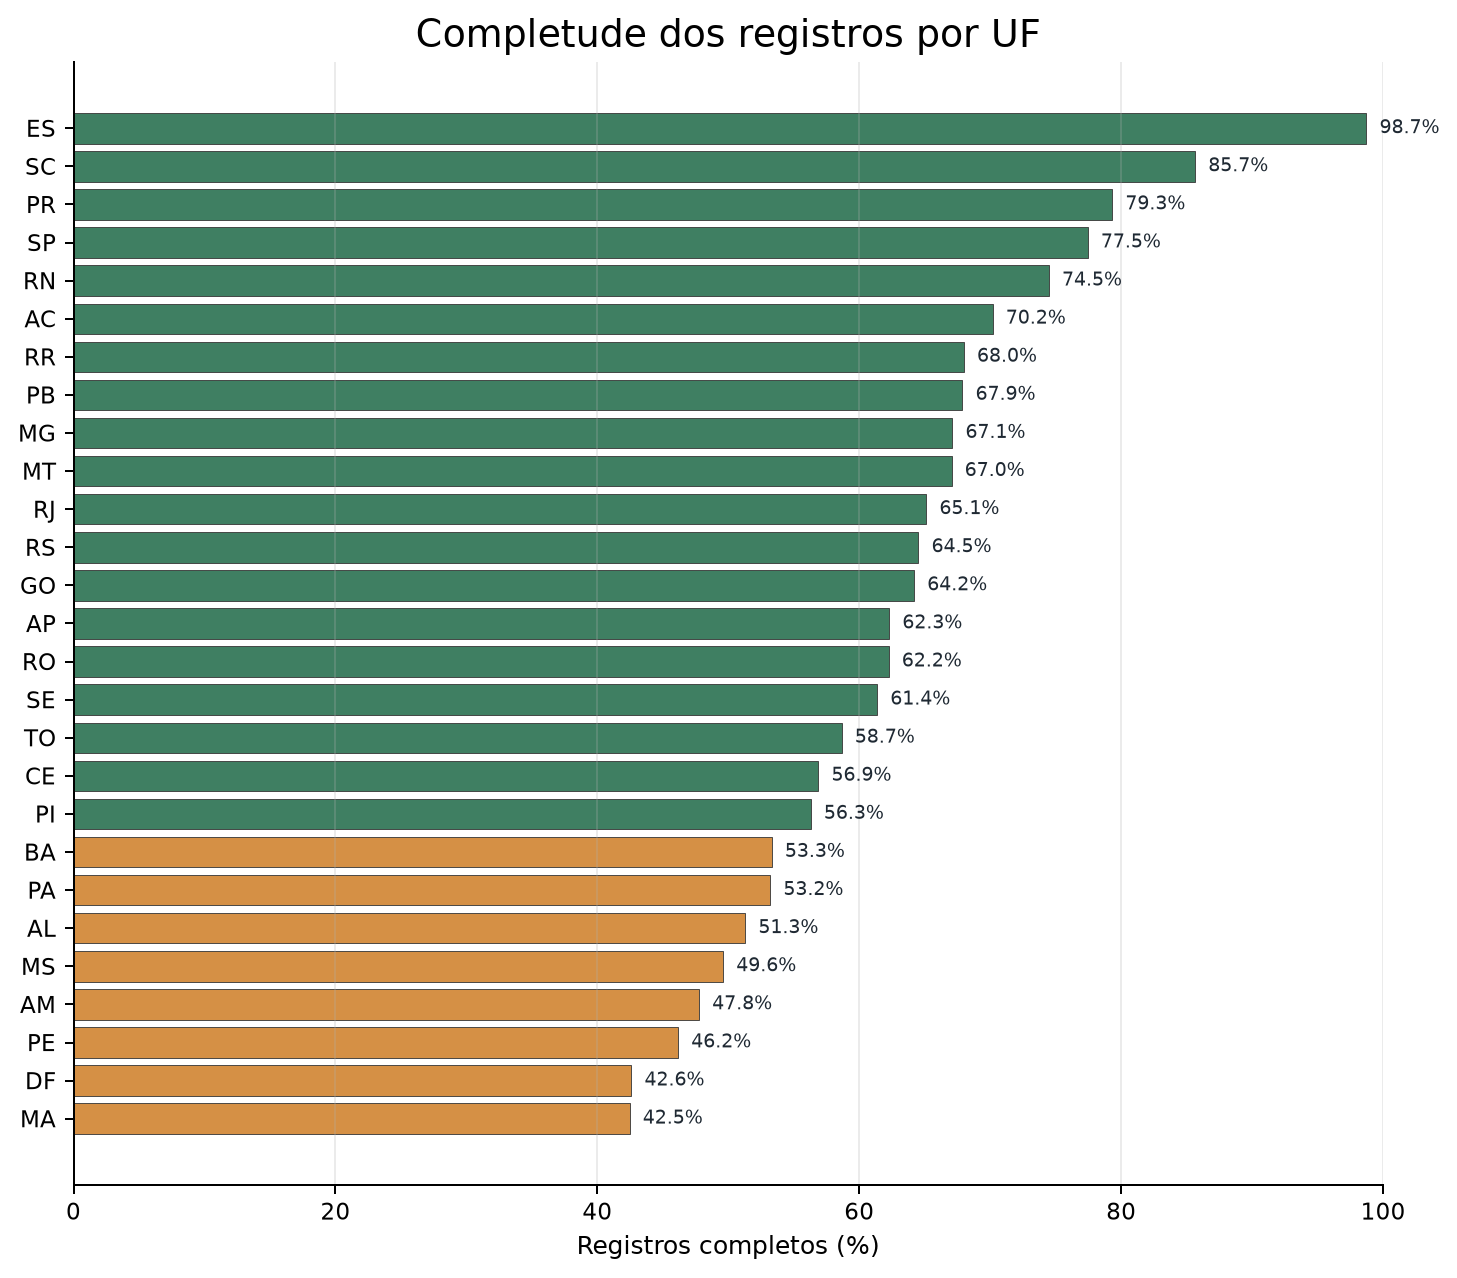
\includegraphics[width=0.82\linewidth]{figures/data_quality.png}
\caption{Percentual de registros completos por unidade federativa na execução completa de 2025. As barras em verde representam UFs com maior completude relativa, enquanto as barras em laranja destacam UFs com menor completude.}
\label{fig:data-quality}
\end{figure}

A Figura~\ref{fig:data-quality} evidencia diferenças territoriais na completude dos registros. Embora a completude global tenha sido de 65,19\%, algumas unidades federativas apresentaram percentuais substancialmente inferiores. Esse resultado demonstra a utilidade dos relatórios de qualidade segmentados, pois permite que pesquisadores considerem limitações de preenchimento antes de realizar comparações estaduais.

O projeto também inclui testes automatizados para verificar a criação do DuckDB, a geração de agregados, a ausência de campos sensíveis na camada Parquet, o funcionamento do enriquecimento geográfico e a validade estrutural dos notebooks. Esses testes aumentam a confiabilidade da pipeline e facilitam sua manutenção.

\section{Potencial de Reuso e Limitações}

O VacinaBR-PNI pode ser reutilizado em diferentes cenários de pesquisa, ensino e gestão. Exemplos incluem análise temporal de doses aplicadas, comparação de registros por UF ou município, estudo da distribuição de tipos de vacina, avaliação de completude dos registros, construção de painéis e ensino de pipelines de dados em saúde pública.

O enriquecimento geográfico amplia o potencial de reuso em análises espaciais, permitindo visualização municipal e cruzamento com outras bases territoriais. Por exemplo, os campos de município podem ser associados a coordenadas e usados em mapas interativos para identificar concentração territorial de registros, diferenças regionais e possíveis lacunas de cobertura operacional. Na execução completa, 5.571 municípios puderam ser mapeados, correspondendo a 168.084.354 registros, ou 98,57\% das doses processadas. Essa visualização deve ser interpretada como uma análise dos registros com município conhecido. Registros sem UF, sem código municipal ou com código incompatível permanecem no conjunto de dados para fins de transparência e qualidade, mas não entram em mapas municipais. A presença de Parquet e DuckDB facilita consultas em ambientes locais, notebooks e ferramentas analíticas sem necessidade de infraestrutura complexa.

\begin{figure}[ht]
\centering
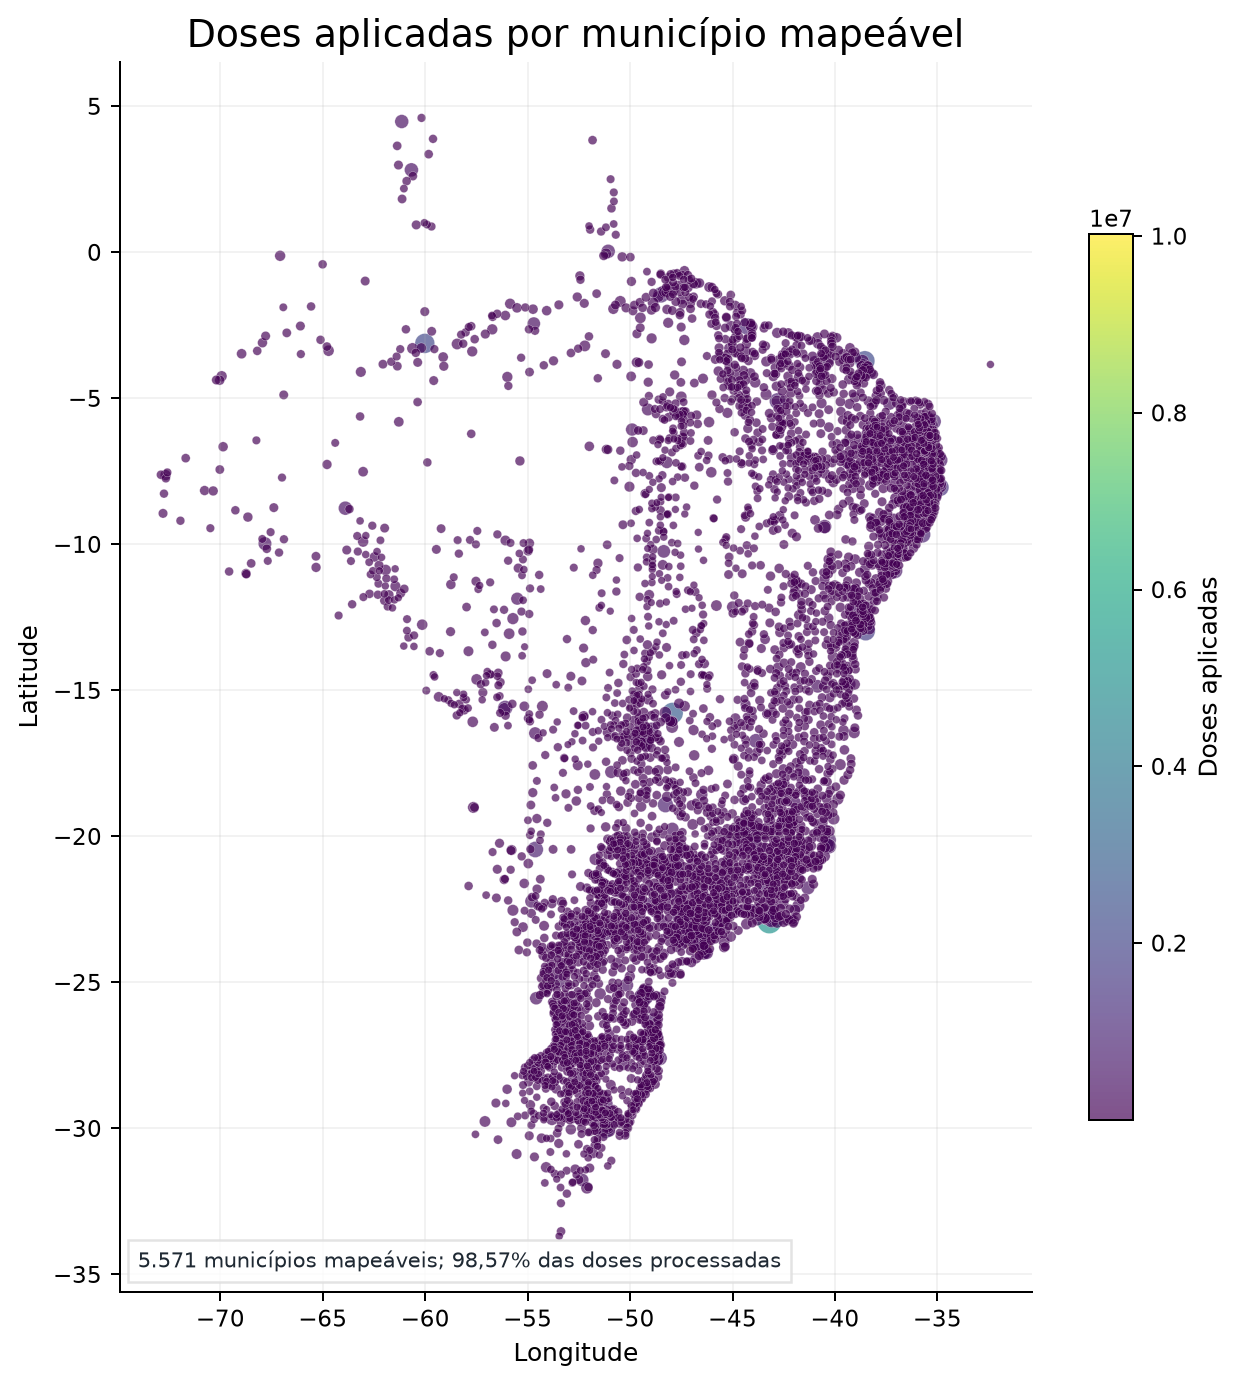
\includegraphics[width=0.75\linewidth]{figures/municipality_map.png}
\caption{Exemplo de uso geográfico do conjunto de dados em nível municipal.}
\label{fig:municipality-map}
\end{figure}

Como limitações, o conjunto de dados depende da qualidade e da disponibilidade da fonte original. A ausência de determinados campos, inconsistências de preenchimento, mudanças no layout dos arquivos CSV e atrasos na publicação mensal podem afetar a curadoria. Além disso, a remoção de identificadores sensíveis limita análises longitudinais em nível individual, mas é necessária para reduzir riscos de privacidade. Outra limitação prática é o volume da camada Parquet na execução anual completa. Por esse motivo, o projeto diferencia os artefatos leves, como CSVs analíticos, documentação e notebooks, dos dados completos em nível de registro.

\section{Disponibilização e Licenciamento}

O pacote de disponibilização é publicado no Zenodo, plataforma que permite atribuição de DOI, controle de versão, metadados bibliográficos e licença explícita para conjuntos de dados. A pasta de disponibilização inclui dados processados, CSVs analíticos, banco DuckDB, documentação, notebooks de exemplo, arquivo de citação e licença. A versão publicada do conjunto de dados é identificada pelo DOI \url{https://doi.org/10.5281/zenodo.21271031}, utilizado como referência persistente para citação e reuso.

Como os Parquets completos atingem vários gigabytes na execução anual, o pacote de dados reúne a camada processada completa, os agregados analíticos, os relatórios de qualidade e os artefatos necessários para interpretação e reprodução do processamento. O fluxo oficial de geração do conjunto de dados é documentado no notebook Colab \texttt{vacinabr\_pni\_colab\_drive\_etl.ipynb}. Dessa forma, usuários que precisam de análises em nível de registro podem consultar os Parquets completos, enquanto usuários interessados em exploração rápida podem utilizar apenas os agregados.

\begin{table}[ht]
\centering
\caption{Artefatos disponibilizados publicamente.}
\label{tab:release-artifacts}
\begin{tabular}{p{4.8cm}p{6.4cm}}
\toprule
\textbf{Artefato} & \textbf{Finalidade} \\
\midrule
\texttt{data/processed/} & Parquets curados em nível de registro, particionados por ano e mês, indicados para pesquisa e consultas analíticas detalhadas. \\
\texttt{data/analytics/} & CSVs agregados para planilhas, BI, apresentações e exploração rápida. \\
\texttt{data/vacinabr\_}\\
\texttt{pni.duckdb} & Banco analítico portátil para consultas SQL sobre Parquet e tabelas materializadas. \\
\texttt{docs/} & Dicionário, esquema, validação, catálogo e metadados de proveniência. \\
\texttt{notebooks/} & Exemplos de consulta, exploração e avaliação da qualidade dos dados. \\
\texttt{requirements.txt} & Dependências Python necessárias para reprodução dos notebooks. \\
\texttt{CITATION.cff} & Citação padronizada do conjunto de dados. \\
\texttt{LICENSE} & Condições de uso, redistribuição e atribuição, preferencialmente com licença aberta compatível com dados derivados de fonte pública. \\
\bottomrule
\end{tabular}
\end{table}

O licenciamento respeita os termos da fonte original e indica claramente que o VacinaBR-PNI é um conjunto de dados derivado dos dados abertos publicados pelo Ministério da Saúde. O pacote adota licença aberta compatível com reuso acadêmico e exige atribuição à fonte original e ao processo de curadoria. O arquivo \texttt{CITATION.cff} fornece uma citação padronizada para facilitar o reuso acadêmico e a identificação da versão publicada.

\section{Conclusão}

Este artigo apresentou o VacinaBR-PNI, um conjunto de dados curado, documentado e enriquecido para análises de doses aplicadas pelo Programa Nacional de Imunizações. A proposta transforma arquivos brutos mensais em uma base analítica reprodutível, com armazenamento em Parquet, consultas via DuckDB, agregados CSV, metadados, dicionário de dados e relatórios de qualidade.

Ao reduzir barreiras de acesso e interpretação dos dados originais, o VacinaBR-PNI contribui para pesquisas epidemiológicas, análises territoriais, construção de painéis e atividades educacionais em ciência de dados. Como trabalhos futuros, pretende-se expandir exemplos de consulta, automatizar novas execuções anuais e integrar fontes auxiliares de contexto socioeconômico e territorial.

\bibliographystyle{plain}
\bibliography{references}

\end{document}
